\documentclass[a4paper,12pt]{report}
\addtolength{\oddsidemargin}{-1.cm}
\addtolength{\textwidth}{2cm}
\addtolength{\topmargin}{-2cm}
\addtolength{\textheight}{3.5cm}
\newcommand{\HRule}{\rule{\linewidth}{0.5mm}}
\setcounter{secnumdepth}{6}
\setcounter{tocdepth}{4}
\makeindex

\usepackage{longtable}
\usepackage{graphicx}
\usepackage{makeidx}
\usepackage{hyperref}
\usepackage{verbatim}
\usepackage{placeins}
\usepackage{float}
\usepackage{titlesec}

\makeatletter
\newcounter{subsubparagraph}[subparagraph]
\renewcommand\thesubsubparagraph{%
  \thesubparagraph.\@arabic\c@subsubparagraph}
\newcommand\subsubparagraph{%
  \@startsection{subsubparagraph}    % counter
    {6}                              % level
    {\parindent}                     % indent
    {3.25ex \@plus 1ex \@minus .2ex} % beforeskip
    {-1em}                           % afterskip
    {\normalfont\normalsize\bfseries}}
\newcommand\l@subsubparagraph{\@dottedtocline{6}{10em}{5em}}
\newcommand{\subsubparagraphmark}[1]{}
\makeatother

\hypersetup{
    colorlinks=true,
    linkcolor=blue,
    filecolor=magenta,      
    urlcolor=cyan,
}


% define the title
\author{Ambitious Design}
\title{ Software Requirements Specifications and Technology Neutral Process Design}
\begin{document}
\setlength{\parskip}{6pt}

% generates the title
\begin{titlepage}

\begin{center}
% Upper part of the page           
\textsc{\LARGE Willburg Outdoor PTY(ltd.)}\\[1.5cm]
\textsc{\Large Smart Image Identifier }\\[1.0cm]
\textsc{\Large Version 1.0 }\\[0.5cm]
% Title
\HRule \\[0.4cm]
{ \huge \bfseries  Software Requirements Specifications and Technology Neutral Process Design}\\[0.4cm]
\HRule \\[0.4cm]
% Author and supervisor
\begin{minipage}{0.4\textwidth}
\begin{flushleft} \large
\emph{Author:}\\
Stephen {Swanepoel}
\end{flushleft}
\end{minipage}
\begin{minipage}{0.4\textwidth}
\begin{flushright} \large
\emph{} \\
u11032091
\end{flushright}
\end{minipage}
\begin{minipage}{0.4\textwidth}
\begin{flushleft} \large
Dian {Veldsman}
\end{flushleft}
\end{minipage}
\begin{minipage}{0.4\textwidth}
\begin{flushright} \large
\emph{} \\
u12081095
\end{flushright}
\end{minipage}

{\large \today}
\end{center}
\end{titlepage}
\footnotesize
\normalsize

\renewcommand{\thesection}{\arabic{section}}
\newpage
\begin{center}
\textsc{\LARGE Software Requirements Specification}\\[1.5cm]
\end{center}

\section{Introduction}
This document aims to set out the functional and non-functional requirements of a system as specified by the Willburg Outdoor PTY(ltd.). The system is required to assess an image by sorting the image into baskets and groupings and then identify if a human is present in the picture. The document will also serve the purpose of communicating the requirements and specifications as needed by the client.

 \subsubsection{Vision}
 The client for this project, Willburg Outdoor PTY(ltd.), has called for the design of an application that will assess an images, identify a human(s) in the image and send the result back as a response to the server based on the outcome of the image which was processed.

\subsubsection{Background}\hfill \break
Willburg Outdoor is company that is passionate about South Africa. With this passion comes the need to protect its farmers and it animals from those who intend to harm them. The client intends to use the system to assist in fighting the following problems: animal poaching and farm attacks. 
Willburg provides its' clients with a camera system which is interfaced with a dashboard as well as a mobile application. The cameras snap pictures when movement is detected and sends them to the Willburg server. The images are then pushed to the respective users. Willburg intend on providing its' users with real-time push notifications when a human has been detected in an image captured by a camera on their property. Smart Image Identifier will play an influential role in the prevention of both farm attacks as well as poaching.

\section {Software architecture overview}

	\begin{figure}[htb]
		\centering
		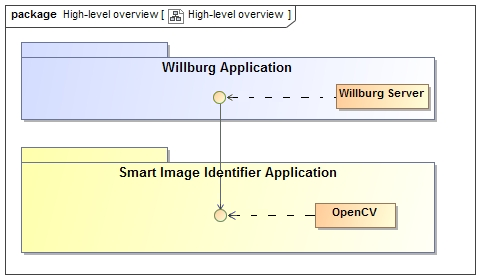
\includegraphics [height= 8cm, width=10cm]{../Diagrams/SystemOverview.png}
		\caption{A high-level overview of the software architecture of the Smart Image Identifier}
	\end{figure}


\section {Overall Software architecture}	
\subsection{Architecture Requirements}
\subsubsection{Access and Integration Requirements}
Any and all interactions by the user will be done through the Willburg Application - this is an application previously designed by the project owner for mobile platforms. All user interactions fall outside of our project scope. 
\subsubsection{Quality Requirements}
	\paragraph {Critical}
		\subparagraph{Performance requirements and tactics}
			\hfill \break
			\hfill \break
			\textbf{Requirements}
			\begin{itemize}
				\item Images which are processed are resized to improve detection as well as the speed at which they are processed by the server.
				\item The system has been created with the most minimal and efficient coding practices possible, given that the result must still be reliable and robust.
				\item The system needs to perform the processing of image as well as the identification of humans in under 2 seconds.
			\end{itemize}
			\hfill \break
			\textbf{Tactics}
				\begin{enumerate}
					\item Thread pooling occurs when a request is received. If a thread is available, it is given to the request for handling. A queue structure is used to handle the thread pooling such that it will add a thread to the pool once the request is complete and pull a thread when there is an incoming request.
					\item Threads are used to run multiple requests to inorder to spread the load accross time.
				\end{enumerate}		
		\subparagraph{Scalability requirements and tactics}
			\hfill \break
			\hfill \break
			\textbf{Requirements}
				\begin{itemize}
					\item Modular programming has be used in order to ensure that there are no restrictions in terms of the systems ability to be extended and improved upon at later stages. It also ensures easy testing of core functionality.
					\item The server should be able to process multiple images at once to ensure the real-time restriction is met for all clients of Willburg.
					\item The system should be able to perform correctly even while under strain due to bulk processing without any loss of data and ensuring the real-time restriction is met.
				\end{itemize}
			\hfill \break	
			\textbf{Tactics}
				\begin{enumerate}
					\item As stated in the previous section threads and thread pooling will be used to handle multiple request within the shortest amount possible. This will ensure that system is able to handle an increase in load without impact on the performance of the system.
					\item Queueing is used to handle requests when the system is in high demand to ensure that no request is lost.
				\end{enumerate}
				
			\subparagraph{Integratibility requirements and tactics}
				\hfill \break
				\hfill \break
				\textbf{Requirements}
					\begin{itemize}
						\item The system will intergrate with the exisiting Willburg architecture and 
					\end{itemize}
				
				\hfill \break
				\textbf{Tactics}
					\begin{enumerate}
						\item The system is designed to support pluggable adapters to allow remote services to use to use the system.
					\end{enumerate}

			\subparagraph{Auditability}
				\hfill \break
				\hfill \break
				\textbf{Requirements}
					\begin{enumerate}
						\item All images processed will be logged and traceable(user, date, time etc.) once pushed into the database.
					\end{enumerate}
				\hfill \break	
				\textbf{Tactics}
					\begin{enumerate}
						\item Auditability will be implemented within the system via a log which will contain all transactions processed by the system. The application server will support specifying logging logic (advices) as crosscutting concerns within aspects or at least provide the ability to apply logging via interception.
						\item Interception is used for auditability to ensure the system contains a full log of all events and details about which client launched the event. This will be useful in ensuring a response may linked to the respective client.
					\end{enumerate}



	\paragraph {Nice-to-have}

		\subparagraph{Flexibility requirements}
			\hfill \break
			\hfill \break
			\textbf{Requirements}
				\begin{itemize}
					\item The system should be able to perform correctly even while under strain due to bulk processing without any loss of data.
					\item The system should be modularized to ensure both easy testing of components as well as addition of components without affecting the system.
				\end{itemize}

		\subparagraph{Maintainability requirements}
			\hfill \break
			\hfill \break
			\textbf{Requirements}
				\begin{itemize}
					\item The system should be designed in technologies which offer user support and continuous updates for extra functionality.
					\item The system must be well structured and documented to ensure future developers are able to understand and maintain the system.
					\item The modular design of the system must be such that if changes must be made to a part of the system, only that part itself should be changed.
				\end{itemize}
		
		\subparagraph{Reliability requirements}
			\hfill \break
			\hfill \break
			\textbf{Requirements}
				\begin{itemize}
					\item The system must be thoroughly tested on the server side, to ensure it will not cause faults or problems.
					\item The notification warning users will receive must be sent out immediately after the image has been processed in a real-time manner.
				\end{itemize}
		
			
\subsubsection{Architectural responsibilities}


\subsubsection{Architectural constraints}
\paragraph{Architeture Constraint}
\begin{enumerate}
	\item Higher level layers can interact with layers below but lower levels should never interact with levels above.
\end{enumerate}
\paragraph{Design Constraint}
\begin{enumerate}
	\item All application software will be modularized into classes using object-oriented design principles.
\end{enumerate}
\paragraph{Implementation Constraint}
\begin{enumerate}
	\item All software components of the application shall be programmed in Java programming language.
\end{enumerate}

\newpage

\subsection {Architecture design}
This section specifies the very high-level software architecture design, i.e. the software architecture
design for the first level of granularity. It includes the allocation of architectural responsibilities to
architectural components, any tactics which should be used at the current level of granularity to
address quality requirements

\subsubsection {Architectural components addressing architectural responsibilities}
	\begin{figure}[htb]
		\centering
		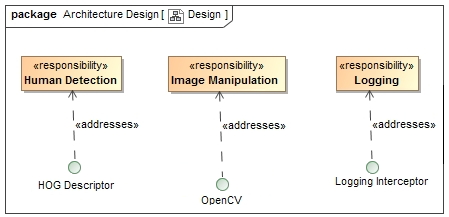
\includegraphics [scale=0.5]{../Diagrams/applicationServerResponsibiltiesAllocationZ.png}
		\caption{PlaceHolder}
	\end{figure}

\subsubsection {Infrastructure}
The layered architectural pattern provides an infrustructure which limits access of components within one layer to components which are either in the same or the next lower level layer. One of the strengths is that a layer can be easily replaced. In particular, one can add further access channels without changing any lower level layers within the software system.


\section {Image Processing System Architecture}
This section specifies the requirements and design of the software architecture second level of granularity. The image processing service is responsible for the manipulation of an image and the detection of a human.

	\subsection {Application server}
	This section specifies the the software architecture requirements and design for the application server
		\subsubsection {Software architecture requirements}
		The architectural requirements include the refined quality requirements and the architectural responsibilities. The architectural constraints for this lower level component are the same as for the system as a whole.
		
			\paragraph {Access and Integration Requirements}
				\subparagraph {Access Channel Requirements}
					The application server will address the first interaction between the existing server and the application. 
				\subparagraph {Integration Channel Requirements}
					The server application must integrate with the image procsessing system in order for images to be pulled from the server.	
			
			\FloatBarrier
			\paragraph {Architectural responsiblities}
				\hfill \break
				The architectural responsibilities of the 	application server
				\begin{figure}[H]
					\centering
					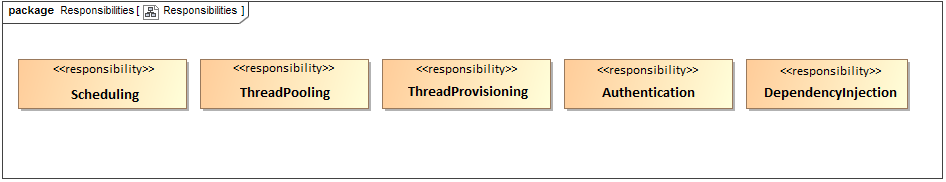
\includegraphics  [scale=0.5]{../Diagrams/applicationServerResponsibiltiesZ.png}
					\caption{The architectural responsibilities of the application server}
				\end{figure}		
		
		\subsubsection {Architecture design}	
			\FloatBarrier	
			\paragraph {Architectural components}
			\hfill \break
				The architectural responsibility allocation the application server			
				\begin{figure}[htb]
					\centering
					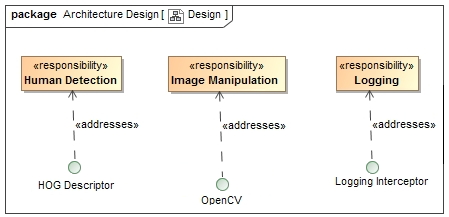
\includegraphics [scale=0.5]{../Diagrams/applicationServerResponsibiltiesAllocationZ.png}
					\caption{The abstract components to which the architectural responsibilities are assigned}
				\end{figure}
			
			\paragraph {Application component concepts and constraints}
			The central concept which will be used to specify application logic (the business processes) are the
			concepts of:
				\begin {itemize}
					\item a \textit{service contract} which encodes the requirements for a service
					\item a \textit{service} which encodes the concrete implementation of a service. 
				\end {itemize}
			These services which encapsulate the processes will be constrained to be stateless, i.e. no state
			is maintained across service requests.
			Long living state is maintained in domain objects which are typically persisted and which should
			not have any business logic.
			
			\paragraph {Frameworks and technologies}
			\hfill \break
			The Spring Framework is an application framework and inversion of control container for the Java platform. The framework's core features can be used by any Java application, but there are extensions for building web applications on top of the Java EE platform. Although the framework does not impose any specific programming model, it has become popular in the Java community as an alternative to, replacement for, or even addition to the Enterprise JavaBeans (EJB) model. The Spring Framework is open source.
			
				\subparagraph {Concrete realization of architectural components}
				\hfill \break
				The Java-EE reference architecture addresses largely all the architectural responsibilities assigned to the application server.
				
				\subparagraph {Tactics}
				\hfill \break
				With the exception of full aspect-oriented programming, Java-EE-7 supports all architectural tactics specified in the software architecture design for the application server.
				
			\paragraph {Concrete realization of flexibility tactics  within Java-EE}
			\hfill \break
			Java-EE supports
				\begin {itemize}
					\item Java-EE is a component-based framework requiring decoupling through interfaces/contracts.
					\item Hot-deployment is supported by most application servers including the most widely used
			open-source application servers like JBoss and Glassfish.
					\item CDI (Context and Dependency Injection) is fully supported within Java-EE with dependency
			injection requested via @Inject annotations.
				\end {itemize}
			
			\paragraph {Concrete realization of maintainability tactics  within Java-EE}
			Java-EE is based on a public standard which is widely supported and hence the support for this technology is secured for the foreseeable future. The technology puts a rigorous framework in place for defining services within stateless session beans which are decoupled through interfaces/contracts. Maintainability is enhanced by dependency injection which allows for changing service providers at any level of granularity without making code changes. Furthermore the replacement of such new
			or improved functionality can be done within a live system using hot deployment.
			
			\paragraph {Concrete realization of reliability tactics  within Java-EE}
			\hfill \break
			Java-EE uses thread-pooling, object-pooling, connection-pooling and clustering to improve scalability.




	\subsection {Image processing}
	This section specifies the the software architecture requirements and design for the image processing application.
		\subsubsection {Software architecture requirements}
		The architectural requirements include the refined quality requirements and the architectural responsibilities. The architectural constraints for this lower level component are the same as for the system as a whole.
		
			\paragraph {Access and Integration Requirements}
				\subparagraph {Access Channel Requirements}
					The image processing application will address the manipulation of images and identification of humans.
				\subparagraph {Integration Channel Requirements}
					The  image processing application must integrate with the image procsessing system in order for images to be processed.	
			
			\FloatBarrier
			\paragraph {Architectural responsiblities}
				\hfill \break
				The architectural responsibilities of the 	application server
				\begin{figure}[H]
					\centering
					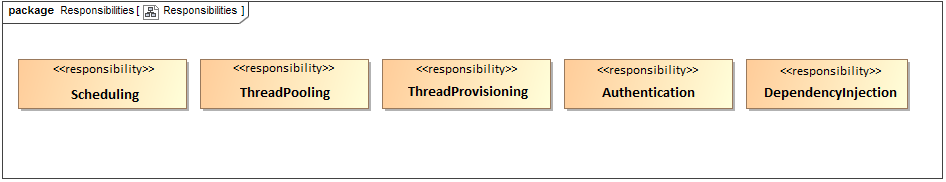
\includegraphics  [scale=0.5]{../Diagrams/applicationServerResponsibiltiesZ.png}
					\caption{The architectural responsibilities of the image processing application}
				\end{figure}		
		
		\subsubsection {Architecture design}	
			\FloatBarrier	
			\paragraph {Architectural components}
			\hfill \break
				The architectural responsibility allocation the application server			
				\begin{figure}[htb]
					\centering
					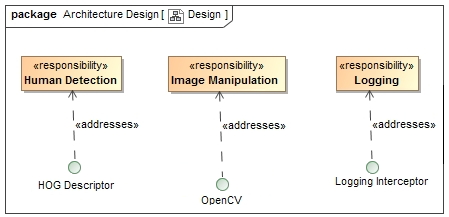
\includegraphics [scale=0.5]{../Diagrams/applicationServerResponsibiltiesAllocationZ.png}
					\caption{The abstract components to which the  image processing applicatio}
				\end{figure}
			
			\paragraph {Frameworks and technologies}
			\hfill \break
			OpenCV (Open Source Computer Vision) is a library of programming functions mainly aimed at real-time computer vision. The library is cross-platform and free for use under the open-source BSD license.
			
				\subparagraph {Concrete realization of architectural components}				
				
					\subsubparagraph {Concrete realization of human detection}
					OpenCV histogram of oriented gradients (HOG) which is a feature descriptor used to detect objects in computer vision and image processing. The HOG descriptor technique counts occurrences of gradient orientation in localized portions of an image - detection window, or region of interest (ROI). OpenCV offers a default implementation in conjunction HOG descriptor to detect humans called \texttt{people\_detection}.
					
					\subsubparagraph {Concrete realization of image manipulation}
						OpenCV has implemented functions that allow image to be manipulated. Such as enlarging the image or grayscaling it. 
				
\end{document}
